\documentclass{article}
\usepackage[top=10px]{geometry}
\usepackage{graphicx}
\usepackage{amsmath,amssymb}
\usepackage[utf8]{inputenc}
\usepackage[T1]{fontenc}
\usepackage[polish]{babel}
\usepackage[fontsize=16pt]{scrextend}

\author{}
\title{Fizyka - Wzory}
\date{}

\begin{document}
	\maketitle
	
	\begin{enumerate}
		
		\item \textbf{Iloczyn wektorowy}:
		\[
		\vec{a} \times \vec{b} = (a_yb_z - a_zb_y)\vec{i} + (a_zb_x - a_xb_z)\vec{j} + (a_xb_y - a_yb_x)\vec{k}
		\]
		
		\item \textbf{Prędkość wektorowa}:
		\[
		\vec{v}_\text{śr} = \frac{\Delta\vec{r}}{\Delta t} = \frac{\vec{r}(t + \Delta t) - \vec{r}(t)}{\Delta t} \quad \left[\frac{\text{m}}{\text{s}}\right]
		\]
		
		\item \textbf{Prędkość średnia}:
		\[
		v_\text{śr} = \frac{x_\text{całk}}{t_\text{całk}} = \frac{\sum \limits_{i=1}^{n}x_i}{\sum \limits_{i=1}^{n}t_i}
		\]
		
		\item \textbf{Prędkość chwilowa}:
		\[
		\vec{v} = \lim_{\Delta t \to 0} \frac{\Delta \vec{r}}{\Delta t} = \frac{d \vec{r}}{dt}
		\]
		\[
		v_x = \frac{dx}{dt}, \quad v_y = \frac{dy}{dt}, \quad v_z = \frac{dz}{dt}
		\]
		
		\item \textbf{Przyspieszenie}:
		\[
		\vec{a}_\text{śr} = \frac{\Delta \vec{v}}{\Delta t}
		\]
		\[
		\quad 
		\vec{a} = \lim_{\Delta t \to 0} \frac{\Delta \vec{v}}{\Delta t} = \frac{d \vec{v}}{dt} = \frac{d^2 \vec{r}}{dt^2}
		\]
		\[
		a_x = \frac{dv_x}{dt}, \quad a_y = \frac{dv_y}{dt}, \quad a_z = \frac{dv_z}{dt}, \quad a_s = \frac{d|\vec{v}|}{dt}, \quad a_n = \frac{v^2}{R}
		\]
		
		\item \textbf{Ruch jednostajny prostoliniowy}:
			\[
			\vec{a} = \vec{0} \implies \vec{v} = \overrightarrow{const} \implies \vec{r}(t) = \vec{r}_0 + \vec{v} \cdot t
			\]
			\text{Dla ruchu wzdłuż osi \(x\)}
			\[
			x(t) = x_0 + v \cdot t
			\]
		
		\item \textbf{Ruch zmienny wzdłuż prostej}:
		\[
		\vec{a} = \overrightarrow{const} \implies \vec{v}(t) = \vec{v}_0 + \vec{a} \cdot t
		\]
		\[\quad \vec{r}(t) = \vec{r}_0 + \vec{v}_0 \cdot t + \frac{\vec{a} \cdot t^2}{2}
		\]
		
		\item \textbf{I zasada dynamiki Newtona}:
		\[
		\vec{F}_w = \vec{0} \iff \vec{v} = \overrightarrow{const}
		\]
		
		\item \textbf{II zasada dynamiki Newtona}:
		\[
		\vec{a} = \frac{\vec{F}_w}{m}
		\]
		
		\item \textbf{Pęd}:
		\[
		\vec{p} = m \cdot \vec{v}
		\]
		
		\item \textbf{III zasada dynamiki Newtona}:
		\[
		\vec{F}_{A \to B} = -\vec{F}_{B \to A}
		\]
		
		\item \textbf{Rzut poziomy}:
		\[
		x(t) = x_0 + v_{0x} \cdotp t = v_0 \cdotp t
		\]
		\[
		y(t) = y_0 + v_{0y} \cdotp t - \frac{gt^2}{2} = H - \frac{gt^2}{2}
		\]
		\[
		t = t_c \text{ dla } y = 0
		\]
		\[
		\quad H - \frac{gt^2}{2} = 0
		\]
		\[
		\quad H = \frac{gt^2}{2} \rightarrow t_c = \sqrt{\frac{2H}{g}} \left[ \sqrt{\frac{m}{\frac{m}{s^2}}} = s \right]
		\]
		\[
		x = z \text{ dla } y = 0
		\]
		\[
		\quad z = v_0 \cdotp t = v_0 \cdotp \sqrt{\frac{2H}{g}} \left[ \frac{m}{s} \sqrt{\frac{m}{\frac{m}{s^2}}} = \frac{m}{s} \cdotp s = m \right]
		\]
		\[
		v_x(t) = \frac{dx}{dt} = v_0 \cdotp 1 \cdotp t^{1-1} = v_0 = const
		\]
		\[
		v_y(t) = \frac{dy}{dt} = - \frac{g}{2} 2t = -gt \left[ \frac{m}{s^2}s = \frac{m}{s} \right]
		\]
		
		\item \textbf{Rzut pionowy}:
		\[
		y(t) = 0 + v_0t - \frac{gt^2}{2}
		\]
		\[
		v_y(t) = \frac{dy}{dt} = v_0 - gt
		\]
		\[
		t = t_c \text{ dla } y = 0 \rightarrow v_0t_c = \frac{g}{2} t_c^2
		\]
		
		\item \textbf{Rzut ukośny}:
		\[
		v_{0x} = v_0 \cdotp \cos\alpha
		\]
		\[
		v_{0y} = v_0 \cdotp \sin\alpha
		\]
		\[
		x(t) = x_0 + v_{0x} \cdotp t = v_0 \cdotp t \cdotp \cos\alpha
		\]
		\[
		y(t) = y_0 + v_{0y} \cdotp t - \frac{gt^2}{2} = v_0 \cdotp t \cdotp \sin\alpha - \frac{gt^2}{2}
		\]
		\[
		v_x(t) = v_{0x} = v_0 \cdotp \cos\alpha
		\]
		\[
		v_y(t) = v_{0y} - g \cdotp t = v_0 \cdotp \sin\alpha - g \cdotp t
		\]
		\[
		t = t_c \text{ dla } y = 0
		\]
		\[
		y(t) = v_0 \cdotp t \cdotp \sin\alpha - \frac{g \cdotp t^2}{2}, \quad v_0 \cdotp t_c \cdotp \sin\alpha - \frac{g \cdotp t_c^2}{2} = 0
		\]
		\[
		t_c \left( v_0 \cdotp \sin\alpha - \frac{g \cdotp t_c}{2} \right) = 0 \Rightarrow t_c = 0 \quad \vee \quad t_c = \frac{2v_0 \cdot \sin\alpha}{g}
		\]
		\[
		z = x(t_c) \longrightarrow \text{z - zasięg}
		\]
		\[
		x(t) = v_0 \cdot t \cdotp \cos\alpha \Rightarrow x(t_c) = v_0 \cdotp \frac{2v_0\sin\alpha}{g} \cdotp \cos\alpha = \frac{2v_0^2 \sin\alpha \cos\alpha}{g}
		\]
		\[
		y = H_{max} \text{ dla } t = t_{wzn}
		\]
		\[
		H_{max} = y(t_{wzn}) = v_0 \cdotp t_{wzn} \cdotp \sin\alpha - \frac{g \cdotp t_{wzn}^2}{2} =
		\]
		\[
		 v_0 \cdotp \frac{v_0 \cdotp \sin\alpha}{g} \cdotp \sin\alpha - \frac{g}{2} \cdotp \left( \frac{v_0 \cdotp \sin\alpha}{g} \right)^2 = \frac{v_0^2 \cdotp \sin^2 \alpha}{g} - \frac{v_0^2 \cdotp \sin^2 \alpha}{2 \cdotp g}
		\]
		\[
		H_{max} = \frac{v_0^2 \cdotp \sin^2 \alpha}{2 \cdotp g}
		\]
		
		\item \textbf{II zasada dynamiki w postaci pędowej}:
		\[
		\overrightarrow{F_{zew}} = \frac{d \vec{p}}{dt}
		\]
		\[
		\Downarrow
		\]
		\[
		\overrightarrow{F_{zew}} = \vec{0} \Rightarrow \frac{d \vec{p}}{dt} = 0 \Leftrightarrow \vec{p} = \overrightarrow{const}
		\]
		\[
		\vec{p}_{pocz} = \vec{p}_{\text{końc}}
		\]
		\[
		\vec{p}_{pocz} = \vec{0}, \quad \vec{p}_{\text{końc}}= m_1 \cdotp \overrightarrow{v_1} - m_2 \cdotp \overrightarrow{v_2} = \vec{0}
		\]
		
		\item \textbf{Energia}:
		\text{Energia kinetyczna}
		\[
		E_k = \frac{mv^2}{2}
		\]
		\text{Energia potencjalna}
		\[
		E_p = -G \frac{Mm}{r}
		\]
		\text{W pobliżu pow. Ziemi}
		\[
		E_p = mgh
		\]
		\text{Siła elektrostatyczna (Coulomba)}
		\[
		E_p = \frac{1}{4 \pi \varepsilon_0} \frac{q_1 q_2}{r}
		\]
		\text{Siła sprężystości}
		\[
		E_p = \frac{kx^2}{w}
		\]
		\text{Energia kinetyczna ruchu obrotowego}
		\[
		E_{koi} = \frac{m_i v_i^2}{2} = \frac{m_i r_i^2 \omega^2}{2}
		\]
		\[
		E_{ko} = \sum\limits_{i = 1}^n \frac{m_i r_i^2 \omega^2}{2} = \frac{1}{2} \omega^2 \sum\limits_{i = 1}^n m_i r_i^2
		\]
		\[
		E_{ko} = \frac{I \omega^2}{2}
		\]
		\item \textbf{Praca}:
		\[
		W = \vec{F} \circ \vec{s} = F \cdot s \cdot \cos a
		\]
		\[
		\Delta W_i = F_i \cdot \Delta x
		\]
		\[
		W = \sum\limits_{i = 1}^n F_i \cdot \Delta x
		\]
		\[
		W = \lim\limits_{\Delta x \rightarrow 0} \sum\limits_{i = 1}^n F_i \cdot \Delta x = \int\limits_{x_1}^{x_2} F(x)dx
		\]
		\[
		x = v_0 \cdot t + \frac{a \cdot t^2}{2}
		\]
		\[
		v = v_0 + a \cdot t \Rightarrow a = \frac{v - v_0}{t}
		\]
		\[
		x = \frac{v + v_0}{2} \cdot t
		\]
		\[
		W = F \cdot x = m \cdot a \cdot x = m \left( \frac{v - v_0}{t} \right) \left( \frac{v + v_0}{2} \right)t = \frac{mv^2}{2} - \frac{mv_0^2}{2}
		\]
		\[
		W = E_k - E_{k_0} \longrightarrow \text{Równoważność pracy i energii}
		\]
		\item \textbf{Moc}:
		\[
		P_{śr} = \frac{\Delta W}{\Delta t}
		\]
		\[
		P = \lim\limits_{\Delta t \rightarrow 0} \frac{\Delta W}{\Delta t} = \frac{dW}{dt}
		\]
		\[
		P = \frac{dW}{dt} = \frac{\vec{F} \circ d \vec{s}}{dt} = \vec{F} \circ \vec{v}
		\]
		\item \textbf{Tarcie}:
		\[
		T_k = \mu_k \cdot N
		\]
		\[
		\mu_s \geq \mu_k
		\]
		\[
		T_s = -F
		\]
		\[
		0 < T_s < T_{\text{smax}}
		\]
		\[
		T_{\text{smax}} = \mu_s \cdot N
		\]
		
		\text{Dla małych prędkości obiektu (wzór Stokesa):}
		$
		\\
		F = 6 \pi \eta r v \longrightarrow \text{Siła oporu kuli o promieniu } r \\
		\eta \rightarrow \text{lepkość płynu}, v \rightarrow \text{prędkość poruszającego się obiektu} \\
		\text{Dla dużych prędkości obiektu (wzór Newtona):} \\
		F = C_x \cdot \frac{\rho v^2}{2} \cdot S, 
		\rho \rightarrow \text{gęstość płynu}, S \rightarrow \text{powierzchnia obiektu} \\
		C_x \rightarrow \text{współczynnik oporu płynu zależny od kształtu obiektu}
		$
		
		\item \textbf{Siły}:
		\[
		\vec{F}_b = -m \cdot \vec{a}_u
		\]
		\[
		\overrightarrow{F_{\text{bezwł}}} = -m \overrightarrow{a_{\text{ukł odn}}}
		\]
		\[
		\overrightarrow{F_{\text{całk}}} = \overrightarrow{F_{\text{oddz}}} + \overrightarrow{F_{\text{bezwł}}}
		\]
		\[
		a_d = \frac{v^2}{R} = \omega^2 \cdot R
		\]
		\[
		F_{od} = m \cdot a_d
		\]
		\[
		F_{od} = m \cdot a_d \frac{mv^2}{R}
		\]
		\[
		F_{od} = m \cdot a_d = m \cdot \omega^2 \cdot R
		\]
		\[
		\overrightarrow{F_c} = -2m(\vec{\omega} \times \vec{v}) \longrightarrow \text{Siła Coriolisa}
		\]
		\text{Oddziaływanie grawitacyjne:}
		\[
		\text{Wzór Newtowna}
		\]
		\[
		F = G \frac{m \cdot M}{r^2}, G = 6.67 \cdot 10^{-11} \text{N} \cdot \text{m}^2 / \text{kg}^2
		\]
		$
			\text{Wzór uwzględniający informację o zwrocie i kierunku siły w miejscu} 	\newline 
			\text{wskazanym przez wektor } \vec{r}
		$
		\[
		\vec{F} = G \frac{m \cdot M}{r^3} \vec{r}
		\]
		\[
		\text{Siła grawitacji na powierzchni Ziemi}
		\]
		\[
		F = mg, g = 9.81 \text{m} / \text{s}^2 
		\]
		\text{Oddziaływanie elektromagnetyczne}
		\[
		F_c = \frac{1}{4 \pi \varepsilon_0} \cdot \frac{q_1 q_2}{r^2} \longrightarrow \text{prawo Coulomba}
		\]
		\[
		\overrightarrow{F_L} =  q(\vec{v} \times \vec{B}) \longrightarrow \text{siła Lorentza}
		\]
		\text{Siła wyporu}
		\[
		\overrightarrow{F_w} = -\rho V \vec{g}
		\]
		\text{Siła sprężystości}
		\[
		F = E \cdot \frac{S}{L_0} \cdot \Delta L
		\]
		\[
		\vec{F} = -k \cdot \vec{x}
		\]
		\item \textbf{Środek masy układu ciał}:
		\[
		x_s = \frac{\sum\limits_{i = 1}^N m_ix_i}{\sum\limits_{i = 1}^N m_i},
		y_s = \frac{\sum\limits_{i = 1}^N m_iy_i}{\sum\limits_{i = 1}^N m_i},
		z_s = \frac{\sum\limits_{i = 1}^N m_iz_i}{\sum\limits_{i = 1}^N m_i}
		\]
		\[
		\Downarrow
		\]
		\[
		\vec{r}_s = \frac{\sum\limits_{i = 1}^N m_i \vec{r}_i}{\sum\limits_{i = 1}^N m_i}
		\]
		\[
		\vec{r}_s = \frac{\sum\limits_{i = 1}^N m_i \vec{r}_i}{\sum\limits_{i = 1}^N m_i}
		\overset{\Delta m_i \rightarrow 0}{\Rightarrow}
		 \vec{r}_s = \frac{\int rdm}{\int dm} =
		\frac{1}{m} \int rdm
		\]
		\[
		mx_s = \sum\limits_{i = 1}^N m_i x_i
		\]
		\text{Pierwsze różniczkowanie}
		\[
		m \frac{dx_s}{dt} = \sum\limits_{i = 1}^N m_i \frac{dx_i}{dt},
		mv_{sx} = \sum\limits_{i = 1}^N m_i v_{xi}
		\]
		\text{Drugie różniczkowanie}
		\[
		m \frac{dv_{sx}}{dt} = ma_{sx} = \sum\limits_{i = 1}^N m_i a_{xi}
		\]
		\text{Po uwzględnieniu II zasady dynamiki}
		\[
		ma_{sx} = \sum\limits_{i = 1}^N m_i a_{xi} = \sum\limits_{i = 1}^N F_{xi}
		\]
		\[
		\text{Analogicznie robimy dla osi y i z}
		\]
		\[
		\Downarrow
		\]
		\[
		m \overrightarrow{a_s} = \sum\limits_{i = 1}^N \vec{F}_i
		\]
		\[
		m \vec{a}_s = \sum\vec{F}_{zi} \longrightarrow \text{Równanie ruchu}
		\]
		\item \textbf{Ruch obrotowy punktu materialnego}:
		\[
		s = \Delta\phi \cdot r \longrightarrow \text{droga kątowa}
		\]
		\[
		\frac{ds}{dt} = \frac{d \phi}{dt}
		\Rightarrow
		\vec{\omega} = \frac{d \vec{\phi}}{dt} \longrightarrow \text{prędkość kątowa}
		\]
		\[
		\vec{v} = \vec{\omega} \times \vec{r} \longrightarrow \text{prędkość liniowa punktu A}
		\]
		\[
		\vec{\varepsilon} = \frac{d \vec{\omega}}{dt} \longrightarrow \text{przyspieszenie kątowe}
		\]
		\text{Przyspieszenie styczne i dośrodkowe}
		\[
		\vec{a} = \frac{d \vec{v}}{dt} = \frac{d}{dt} (\vec{\omega} \times \vec{r}) =
		\frac{d \vec{\omega}}{dt} \times \vec{r} + \vec{\omega} \times \frac{d \vec{r}}{dt}
		\]
		\[
		\vec{a}_s = \frac{d \vec{\omega}}{dt} \times \vec{r} = \vec{\varepsilon} \times \vec{r} \Rightarrow | \vec{a}_s | = \left| \frac{d \vec{v}}{dt} \right|
		\]
		\[
		\vec{a}_n = \vec{\omega} \times \frac{d \vec{r}}{dt} = \vec{\omega} \times \vec{v} \Rightarrow | \vec{a}_n | = \frac{v^2}{r}
		\]
		\item \textbf{Moment siły}:
		\[
		\vec{M} = \vec{r} \times \vec{F}, \vec{r} \longrightarrow \text{ramię siły}
		\]
		\[
		\vec{r} \text{ II } \vec{F} \Rightarrow \vec{M} = 0		
		\]
		\[
		M = rF\sin\alpha = r_{\perp} \cdot F
		\]
		\item \textbf{Moment bezwładności}:
		\[
		I = \sum\limits_{i = 1}^n \Delta m_i \cdot r^2_i
		\]
		\[
		I = \lim\limits_{n \rightarrow \infty} \sum\limits_{i = 1}^n \Delta m_i \cdot r_i = \int r^2 dm
		\]
		\text{Twierdzenie Steinera}
		\[
		I = I_0 + md^2
		\]
		\text{II zasada dynamiki dla ruchu obrotowego}
		\[
		\vec{M} = \sum\limits_{i = 1}^n \vec{r_i} \times \vec{F_i}
		\]
		\[
		F_i = \Delta m_i a_i = \Delta m_i \varepsilon r_i
		\]
		\[
		M = \sum\limits_{i = 1}^n r_i F_i = \sum\limits_{i = 1}^n \Delta m_i \varepsilon r_i^2 = \varepsilon \sum\limits_{i = 1}^n m_i r_i^2
		\]
		\[
		M = I \cdot \varepsilon
		\]
		\[
		\vec{M} = I \cdot \vec{\varepsilon}
		\]
		\item \textbf{Moment pędu}:
		\[
		\vec{L_i} = \vec{r_i} \times \vec{p_i} = \vec{r_i} \times \Delta m_i \cdot \vec{v_i}
		\]
		\[
		\vec{L_i} = \Delta m_i \vec{r_i} \times (\vec{\omega} \times \vec{r_i})
		\]
		\[
		\vec{\omega} = \vec{\omega_{\perp}} + \vec{\omega_{\parallel}}
		\]
		\[
		\text{Dla całej bryły: }
		L = \sum\limits_{i = 1}^n r_i \Delta m_i v_i
		\]
		\[
		v = \omega \cdot r
		\]
		\[
		L = \sum\limits_{i = 1}^n r_i \Delta m_i \omega r_i = \omega \sum\limits_{i = 1}^n \Delta m_i r_i^2 = I \omega
		\]
		\[
		\vec{L} = I \vec{\omega}
		\]
		\[
		\vec{L} = \L\vec{L_{\perp}} + \vec{L_{\parallel}} = I_{\perp} \vec{\omega_{\perp}} + I_{\parallel} \vec{\omega_{\parallel}}
		\]
		\[
		I_{\perp} = mr^2, I_{\parallel} = \frac{1}{2} mr^2
		\]
		\text{II zasada dynamiki dla ruchu obrotowego}
		\[
		\vec{M} = I \vec{\varepsilon} = I \cdot \frac{d \vec{\omega}}{dt} = \frac{d(I \cdot \vec{\omega})}{dt}
		\]
		\[
		\vec{M} = \frac{d \vec{L}}{dt}
		\]
		\text{Zasada zachowania pędu}
		\[
		\vec{M} = \frac{d \vec{L}}{dt} \text{ jeżeli } \vec{M} = \vec{0} \Rightarrow \vec{L} = \overrightarrow{const}
		\]
		\[
		L = L' \text{ tzn. } I \omega = I' \omega '
		\]
		\[
		I > I' \Rightarrow \omega ' > \omega
		\]
		\text{Elipsoida bezwładności bryły sztywnej względem jej środka masy}
		\[
		\frac{x^2}{a^2} + \frac{y^2}{b^2} + \frac{z^2}{c^2} = 1
		\]
		\[
		a = \frac{1}{\sqrt{I_x}}, b = \frac{1}{\sqrt{I_y}}, c = \frac{1}{\sqrt{I_z}}
		\]
		\item \textbf{Precesja bąka}:
		\[
		| \vec{M} | = | \vec{r} \times m \vec{g} | = rmg \sin \alpha
		\]
		\[
		r \longrightarrow \text{wektor położenia środka masy przy zetknięciu z podłożem}
		\]
		\[
		d \vec{L} = \vec{M} dt
		\]
		\[
		d \varPhi = \frac{dL}{L \sin\alpha} = \frac{Mdt}{L \sin \alpha}
		\]
		\[
		\omega_p = \frac{d \varPhi}{dt} = \frac{M}{L \sin \alpha} = \frac{mgr \sin \alpha}{L \sin \alpha} = \frac{mgr}{L}
		\]
		\[
		\vec{M} = \vec{\omega_p} \times \vec{L}
		\]
		\item \textbf{Drgania harmoniczne}:
		\[
		m = \frac{d^2x}{dt^2} = -kx
		\]
		\[
		x(t) = A \sin (\omega_0t + \varPhi)
		\]
		\text{A - amplituda, k - współczynnik sprężystości, $\omega_0$ - częstość}
		\text{kołowa drgań, $\varPhi$ - początkowa faza drgań}
		\newline
		\text{Prędkość oscylatora harmonicznego}
		\[
		v(t) = \frac{dx}{dt} A \cdot \omega_0 \cdot \cos(\omega_0 \cdot t + \varPhi)
		\]
		\text{Przyspieszenie oscylatora harmonicznego}
		\[
		a(t) = \frac{d^2 x}{dt^2} = -A \cdot \omega_0^2 \cdot \sin(\omega_0 \cdot t + \varPhi)
		\]
		\[
		a(t) = \frac{d^2x}{dt^2} = -\omega_0^2 \cdot x(t)
		\]
		\[
		\frac{d^2 x}{dt^2} = - \frac{k}{m} \cdot x(t) = - \omega^2_0 \cdot x(t) \Rightarrow \frac{k}{m} = \omega_0^2
		\]
		\text{Wychylenie}
		\[
		x(t) = A \cdot \sin \left(\sqrt{\frac{k}{m}} \cdot t + \varPhi \right)
		\]
		\text{Okres drgań własnych}
		\[
		T = \frac{2 \pi}{\omega} \Longrightarrow T_0 = \frac{2 \pi}{\omega} = 2 \pi \sqrt{\frac{m}{k}}
		\]
		\text{Częstotliwość}
		\[
		f = \frac{1}{T}
		\]
		\text{Energia potencjalna sprężystości}
		\[
		W = \vec{F} \circ \vec{x} = Fx \cdot \cos \alpha
		\]
		\[
		\Delta W = F \cdot \Delta x
		\]
		\[
		W = \lim\limits_{\Delta x \rightarrow 0} \sum\limits_{x_1}^{x_2} F \Delta x = \int\limits_{x_1}^{x_2} Fdx
		\]
		\[
		W = \int\limits_0^x F \cdot dx = \int_0^x (k \cdot x) \cdot dx = \left. \frac{k \cdot x^2}{2} \right|_0^2 = \frac{k \cdot x^2}{2}
		\]
		\[
		W = \Delta E \Rightarrow E_p = \frac{k \cdot x^2}{2}
		\]
		\text{Energia kinetyczna}
		\[
		E_k = \frac{m \cdot v^2}{2} = \frac{m}{2} \cdot \left( \frac{dx}{dt} \right)^2 = \frac{m}{2} \cdot (A \cdot \omega_0 \cdot \cos(\omega_0 \cdot t + \varPhi))^2 
		\]
		\[
		\Downarrow
		\]
		\[
		E_k = \frac{m \cdot \omega_0^2 \cdot A^2}{2} \cdot \cos^2(\omega_0 \cdot t + \varPhi)
		\]
		\newpage
		\text{Energia całkowita}
		\[
		E_c = E_p + E_k = \frac{k \cdot x^2}{2} + \frac{m \cdot \omega_0^2 \cdot A^2}{2} \cdot \cos^2(\omega_0 \cdot t + \varPhi) =
		\]
		\[
		= \frac{k \cdot A^2}{2} \cdot \sin^2(\omega_0 \cdot t + \varPhi) + \frac{k \cdot A^2}{2} \cdot \cos^2(\omega_0 \cdot t + \varPhi) \Rightarrow E_c = \frac{k \cdot A^2}{w}
		\]
		\text{Siła ciężkości}
		\[
		F_s = m \cdot g \cdot \sin \varTheta \longrightarrow \text{Składowa styczna siły ciężkości}
		\]
		\[
		F_r = m \cdot g \cdot \cos \varTheta \longrightarrow \text{Składowa radialna siły ciężkości}
		\]
		\text{Dla małych kątów (<10\textdegree) sin$\Theta \approx \Theta$}
		\[
		\sin \varTheta = \frac{x}{l} \Longrightarrow \varTheta = \frac{x}{l}
		\]
		\[
		F_s = -mg\varTheta = -mg \frac{x}{l} = - \frac{mg}{l}x
		\]
		\[
		x = \frac{mg}{l} = m \omega_0^2 \Rightarrow \frac{g}{l} = \left( \frac{2 \pi}{T_0} \right)^2 \Rightarrow T_0 = 2 \pi \sqrt{\frac{l}{g}}
		\]
		
		\renewcommand{\arraystretch}{1.5}
		
		\begin{table}[h]
			\centering
			\caption{Drgania harmoniczne - wahadło fizyczne}
			\label{tab:Drgania harmoniczne - wahadło fizyczne}
			\begin{tabular}{|c|c|}
				\hline
				\textbf{Punkt materialny} & \textbf{Bryła sztywna} \\
				\hline
				$F = -kx$ & $M -K\alpha$  \\
				\hline
				$F = ma$ & $M = I \varepsilon$ \\
				\hline
				$k = m \omega_0^2$ & $K = I \omega_0^2$ \\
				\hline
				$\omega_0 = \sqrt{\frac{k}{m}}$ & $\omega_0 = \sqrt{\frac{K}{I}}$ \\
				\hline
			\end{tabular}
		\end{table}
		\[
		M = F_sl = -mgl \sin \alpha \approx -mgl \alpha
		\]
		\[
		K = mgl
		\]
		\[
		\omega_0 = \sqrt{\frac{K}{I}}
		\]
		\newpage
		\[
		T_0 = \frac{2 \pi}{\omega_0} = 2 \pi \sqrt{\frac{I}{K}} \Rightarrow T_0 = 2 \pi \sqrt{\frac{I}{mgl}}
		\]
		\begin{figure}[h]
			\centering
			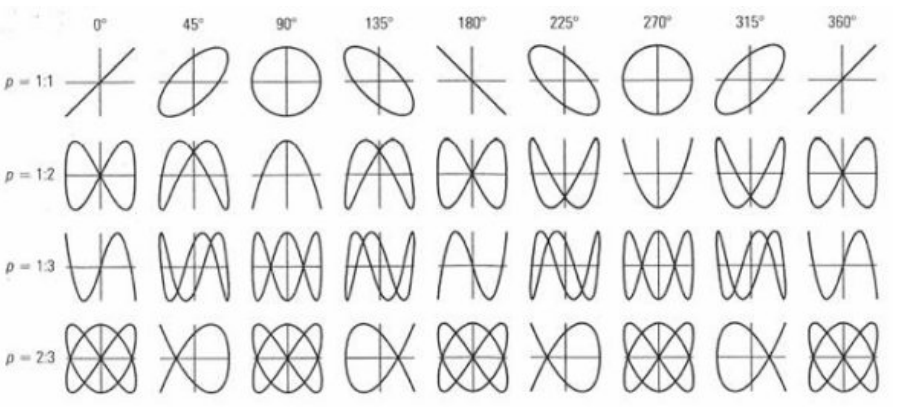
\includegraphics[width=1\textwidth]{krzywe_Lissajous.png}
			\caption{Krzywe Lissajous}
			\label{fig:krzywe_Lissajous}
		\end{figure}
		\text{Składanie drgań równoległych}
		\begin{itemize}
			\item \text{Ta sama częstościach ale różna faza i amplituda}
			\[
			x_1(t) = A_1 \cos(\omega t + \varphi_1)
			\]
			\[
			x_2(t) = A_2 \cos (\omega t + \varphi_2)
			\]
			\[
			x(t) = x_1(t) + x_2(t) = A_1 \cos (\omega t + \varphi_1) + A_2 \cos (\omega t + \varphi_2) =
			\]
			\[
			= A \cdot \cos (\omega t + \varphi)
			\]
			\[
			A = \sqrt{A_1^2 + A_2^2 + 2A_1A_2\cos(\varphi_1 - \varphi_2)}
			\]
			\[
			\tan \varphi = \frac{A_1 \sin \varphi_1 + A_2 \sin \varphi_2}{A_1 \cos \varphi_1 + A_2 \cos \varphi_2}
			\]
			\item \text{Różne częstości} \\
			\textbf{Twierdzenie Fouriera}:
			\[
			x(t) = \frac{1}{2} A_0 + \sum\limits_{k = 1}^\infty [A_k \cos(k \omega t) + B_k \sin (k \omega t)]
			\]
			\newpage
			\item \text{Podobna częstość (dudnienia)}
			\[
			A[\sin (\omega_1 t) + \sin (\omega_2 t)] = A \cos \left( \frac{\omega_1 - \omega_2}{2}t \right) \sin \left( \frac{\omega_1 + \omega_2}{2}t \right)
			\]
		\end{itemize}
		\text{Drgania tłumione}
		\[
		F_t = -bv
		\]
		\[
		m \frac{d^2x}{dt^2} = -b \frac{dx}{dt} -kx
		\]
		\[
		x(t) = A_0e^{-\beta t} \sin (\omega t + \varphi)
		\]
		\[
		\omega = \sqrt{\omega_0^2 - \beta^2}
		\]
		\[
		\beta = \frac{b}{2m}
		\]
		$
		F_t \longrightarrow \text{siła oporu proporcjonalna do prędkości ciała i} \\ \text{przeciwnie do niej skierowana} \\
		A_0e^{-\beta t} \longrightarrow \text{amplituda} \\
		k \longrightarrow \text{współczynnik sprężystości} \\
		\omega_0 \longrightarrow \text{częstość kołowa drgań} \\
		\omega \longrightarrow \text{częstość oscylatora tłumionego} \\
		\varphi \longrightarrow \text{początkowa faza drgań} \\
		b \longrightarrow \text{współczynnik oporu} \\
		\beta \longrightarrow \text{współczynnik tłumienia} \\ \\
		$
		\text{Logarytmiczny dekrement tłumienia}
		\[
		\Lambda = \ln \frac{A_n}{A_{n+1}} = \ln \frac{A(t)}{A(t + T)}
		\]
		\text{Względny współczynnik tłumienia}
		\[
		\zeta = \frac{\beta}{\omega_0}
		\]
		\newpage
		\begin{figure}[h]
			\centering
			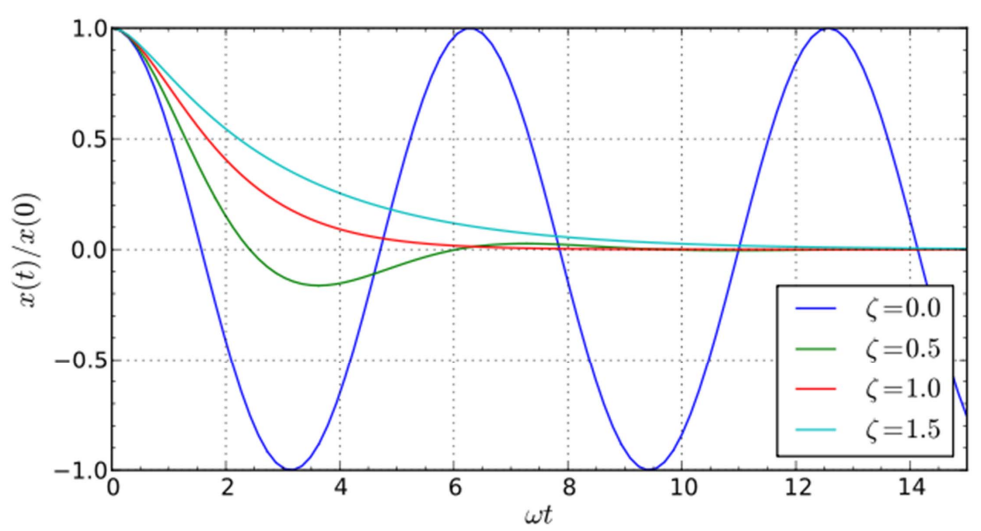
\includegraphics[width=1\textwidth]{drgania_tlumione.png}
			\caption{Drgania tłumione}
			\label{fig:drgania_tlumione}
		\end{figure}
		\text{Drgania wymuszone}
		\[
		m \frac{d^2x}{dt^2} + b \frac{dx}{dt} + kx = F_0 \sin (\Omega t)
		\]
		\[
		x(t) = A \sin (\Omega t + \varphi)
		\]
		\[
		A = \frac{F_0}{m \sqrt{(\omega_0^2 - \Omega^2)^2 + 4 \beta^2 \Omega^2}}
		\]
		\[
		\varphi = \arctan \left( - \frac{2 \beta \Omega}{\omega_0^2 - \Omega^2} \right)
		\]
		\newpage
		\begin{figure}[h]
			\centering
			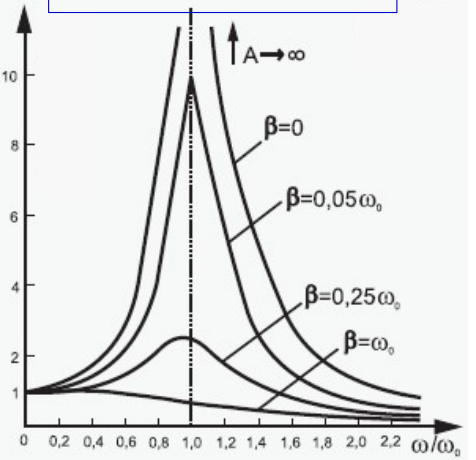
\includegraphics[width=0.5 \textwidth]{drgania_wymuszone.png}
			\caption{Drgania wymuszone}
			\label{fig:drgania_wymuszone}
		\end{figure}
		\item \textbf{Fale}:
		\begin{figure}[h]
			\centering
			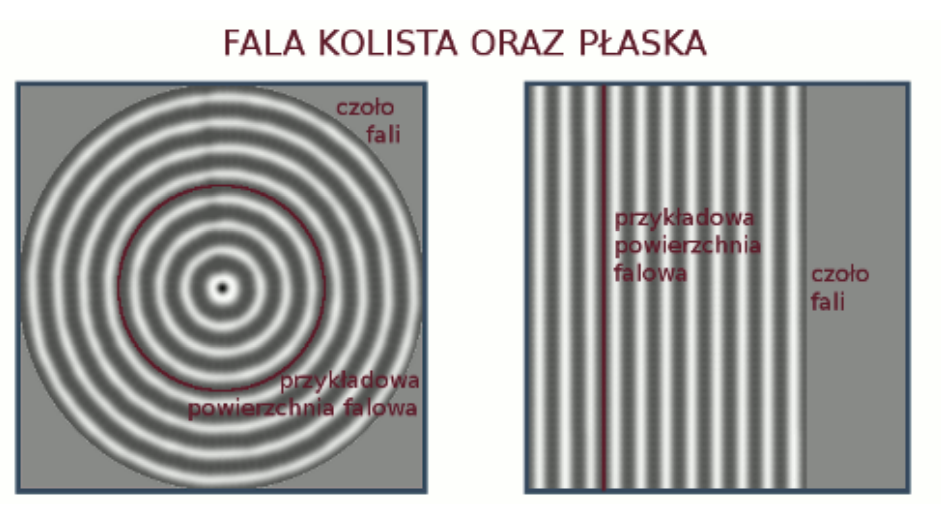
\includegraphics[width=0.75 \textwidth]{fale.png}
			\caption{Fala kulista oraz płaska}
			\label{fig:fale}
		\end{figure}
		\\
		\text{Równanie fali}
		\[
		\varPsi(x, t) = A \sin (kx - \omega t)
		\]
		\[
		k = \frac{2 \pi}{\lambda}, \omega = \frac{2 \pi}{T}
		\]
		\text{Prędkość fali}
		\[
		V_f = \frac{\omega}{k} = \frac{\lambda}{T} = \lambda \cdot f
		\]
		\newpage
		\begin{table}[h]
			\centering
			\caption{Drgania harmoniczne - wahadło fizyczne}
			\label{tab:Fale w ośrodkach sprężystych}
			\begin{tabular}{|c|c|c|c|}
				\hline
				& \textbf{Ciało stałe} & \textbf{Ciecz} & \textbf{Gaz} \\
				\hline
				\text{Fala podłużna} & $V_f = \sqrt{\frac{E}{\rho}}$ & $V_f = \sqrt{\frac{K}{\rho}}$ & $V_f = \sqrt{\frac{\kappa \cdot p}{\rho}}$ \\
				\hline
				\text{Fala poprzeczna} & $V_f = \sqrt{\frac{G}{\rho}}$ & - & - \\
				\hline
			\end{tabular}
		\end{table}
		$
		\rho \longrightarrow \text{gęstość} \\
		E \longrightarrow \text{moduł Younga} \\
		G \longrightarrow \text{moduł sztywności} \\
		K \longrightarrow \text{moduł ściśliwości cieczy} \\
		p \longrightarrow \text{ciśnienie} \\
		\kappa = \frac{C_p}{C_v} \\ \\
		$
		\text{Prędkość grupowa}
		\[
		V_g = \frac{d \omega}{dk}
		\]
		\text{Prawo załamania}
		\[
		n_{21} = \frac{n_2}{n_1} = \frac{\sin \alpha}{\sin \beta} = \frac{V_1}{V_2} = \frac{\lambda_1}{\lambda_2}
		\]
		\text{Interferencja fal}
		\[
		\varPsi_1 = A \sin (kx - \omega t)
		\]
		\[
		\varPsi_2 = A \sin (kx - \omega t + \varphi)
		\]
		\[
		\varPhi = \varPsi_1 + \varPsi_2 = 2A \cos \left( \frac{\varphi}{2} \right) \sin \left( kx - \omega t + \frac{\varphi}{2} \right)
		\]
		\text{Fala stojąca} \\
		$\left.
		\begin{array}{lll}
			\varPsi_1 = A \sin(kx - \omega t) \\
			+ \\
			\varPsi_2 = A \sin(kx -+\omega t)
		\end{array} 
		\right\} \Longrightarrow \varPsi = \varPsi_1 + \varPsi_2 = 2A \sin (kx) \cos (\omega t)$
		\newpage
		\text{Maksima interferencyjne}
		\[
		d \cdot \sin \alpha = n \cdot \lambda
		\]
		\text{Minima interferencyjne}
		\[
		d \cdot \sin \alpha = 2(n - 1) \cdot \frac{\lambda}{2}
		\]
		$
		d \longrightarrow \text{odległość pomiędzy szczelinami} \\
		n = 0, 1, 2, 3, ... \\ \\
		$
		\text{Kąt Brewstera}
		\[
		\tan \alpha_B = n
		\]
		$
		\alpha \longrightarrow \text{kąt padania światła} \\
		n \longrightarrow \text{współczynnik załamania dielektryka} \\ \\
		$
		\text{Efekt Dopplera}
		\begin{itemize}
			\item \text{Źródło zbliża się do obserwatora}
			\[
			\lambda_o = \lambda_z - v_zT, \lambda = \frac{v}{f}, T = \frac{1}{f_z}
			\]
			\[
			\frac{v}{f_o} = \frac{v}{f_z} - \frac{v_z}{f_z} \Rightarrow f_o = f_z \frac{v}{v - v_z}
			\]
			\item \text{Źródło oddala się od obserwatora}
			\[
			\lambda_o = \lambda_z + v_zT, \lambda = \frac{v}{f}, T = \frac{1}{f_z}
			\]
			\[
			\frac{v}{f_o} = \frac{v}{f_z} + \frac{v_z}{f_z} \Rightarrow f_o = f_z \frac{v}{v + v_z}
			\]
		\end{itemize}
		$
		v \longrightarrow \text{prędkość fali} \\
		v_o \longrightarrow \text{prędkość obserwatora} \\
		v_z \longrightarrow \text{prędkość źródła}
		$
		\newpage
		\text{Natężenie dźwięku}
		\[
		I = \frac{P}{S}
		\]
		\[
		I_0 = 10^{-12} \left[ \frac{W}{m^2} \right]
		\]
		\text{Próg bólu}
		\[
		I_B = 1 \left[ \frac{W}{m^2} \right]
		\]
		\text{Poziom natężenia dźwięku}
		\[
		L = 10 \log \frac{I}{I_0} [db]
		\]
	
	\end{enumerate}
	
\end{document}